\begin{frame}{ARCHITETTURE DI RIFERIMENTO}
    Tutti i test sono stati eseguiti su tre architetture differenti in termini di performance, dimensioni e costo.
    \begin{minipage}{\linewidth}
        \hspace{-1cm}
        \begin{minipage}{0.45\linewidth}
            \begin{figure}
                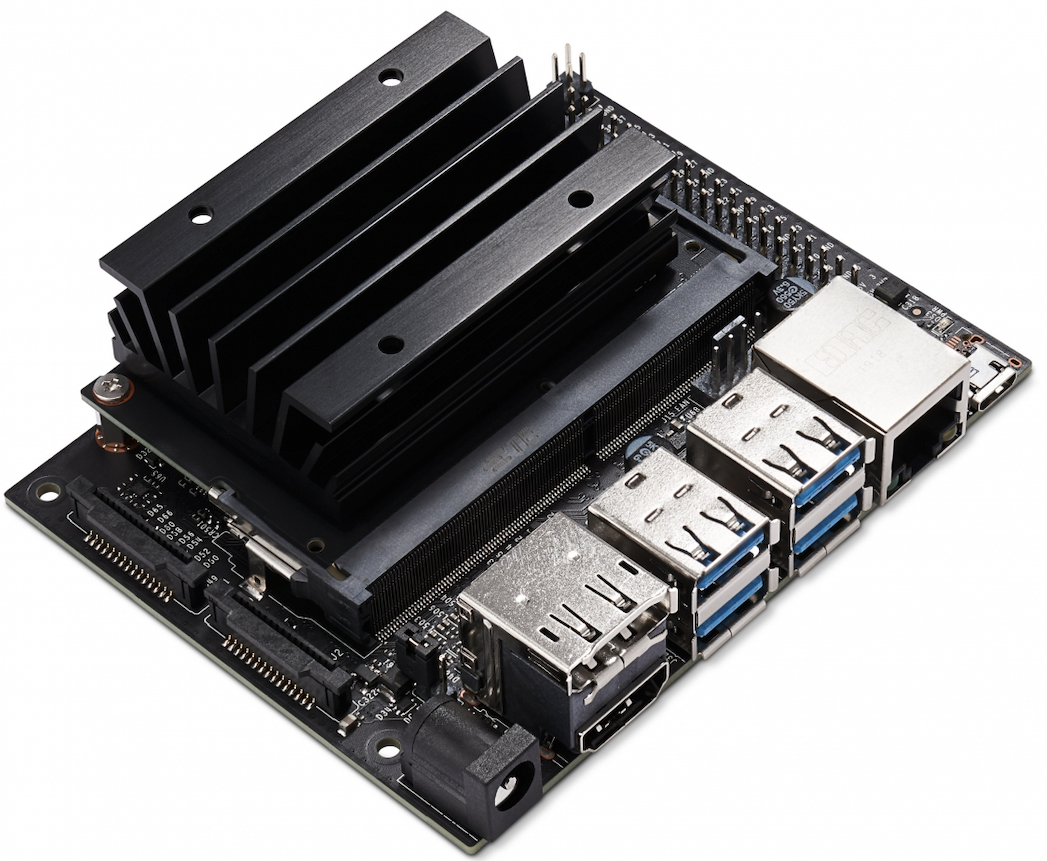
\includegraphics[width = 0.5\linewidth]{jetson1.png}
                \vspace{-0.1cm}
                \caption{NVidia Jetson Nano}
            \end{figure}
            \vspace{-1.3cm}
            \begin{figure}
                
\includegraphics[width = 0.5\linewidth]{colab_logo.png}
                \vspace{-0.6cm}
                \caption{Google Colaboratory}
            \end{figure}
            \vspace{-0.7cm}
            \begin{figure}
                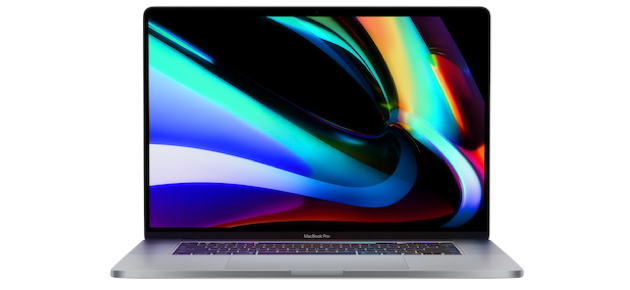
\includegraphics[width = 0.7\linewidth]{MacBook-Pro-16.png}
                \caption{Macbook Pro}
            \end{figure}
        \end{minipage}
        \begin{minipage}{0.65\linewidth}
            \begin{table}
                %\renewcommand{\baselinestretch}{1}
                \centering
                \begin{adjustbox}{max width=\textwidth}
                {\Huge
                \begin{tabular}{|c||c|c|c||}
                    \hline
                    \multirow{2}{*}{\bfseries{ARCHITETTURE}} & \multicolumn{3}{c||}{\bfseries{SPECIFICHE TECNICHE}}\\            & \bfseries{CPU} & \bfseries{GPU} & \bfseries{RAM}\\
                    \hline
                    \hline
                    {\bfseries{JETSON NANO}} & 4 $\times$ ARM Cortex-A57 @ 1.43 GHz & NVidia Maxwell @ 921 MHz & 4 GB 1600 MHz LPDDR4\\
                    \hline
                    {\bfseries{MACBOOK PRO}} & 8 $\times$ Intel Core i9 @ 2.3 GHz & AMD Radeon Pro 5500M @ 8 GB & 32 GB 2667 MHz DDR4\\
                    \hline 
                    {\bfseries{COLAB}} & 2 $\times$ Intel(R) Xeon(R) @ 2.20 GHz & NVidia Tesla P-100 @ 16 GB & 27 GB DDR4\\
                    \hline
                \end{tabular}
                }%
                \end{adjustbox}
                \vspace{0.5cm}
                \caption{Specifiche tecniche delle tre architetture utilizzate.}
                \label{specifiche}
            \end{table}
        \end{minipage}
    \end{minipage}
\end{frame}